\noindent
\subsection{Reviewer based features}
\label{reviewer_analysis}

The success of the peer-review process is immensely dependent on the reviewers as they determine the quality of a paper and, consequently, the quality of the journal. We hence investigate certain reviewer behaviors (pointed out in~\cite{sikdar2016anomalies}) that could  be indicative of his/her performance.

\subsubsection{Accept ratio (RAC)} For each reviewer we define a metric called accept ratio (this is different from the acceptance ratio defined in the previous section) Formally, the {\bf accept ratio} for reviewer $j$ is $accept\,ratio_{j}=\frac{accept_{j}}{accept_{j} + reject_{j}}$ 
where $accept_{j}$ and $reject_{j}$ respectively represent the number of papers reviewer $j$ accepted and rejected. The mean accept ratio across all the reviewers is $0.62$. An accept ratio of 1 for a reviewer would mean that he accepted all the papers that were assigned to him.

\begin{figure*}
\centering
\begin{tabular}{ccc}
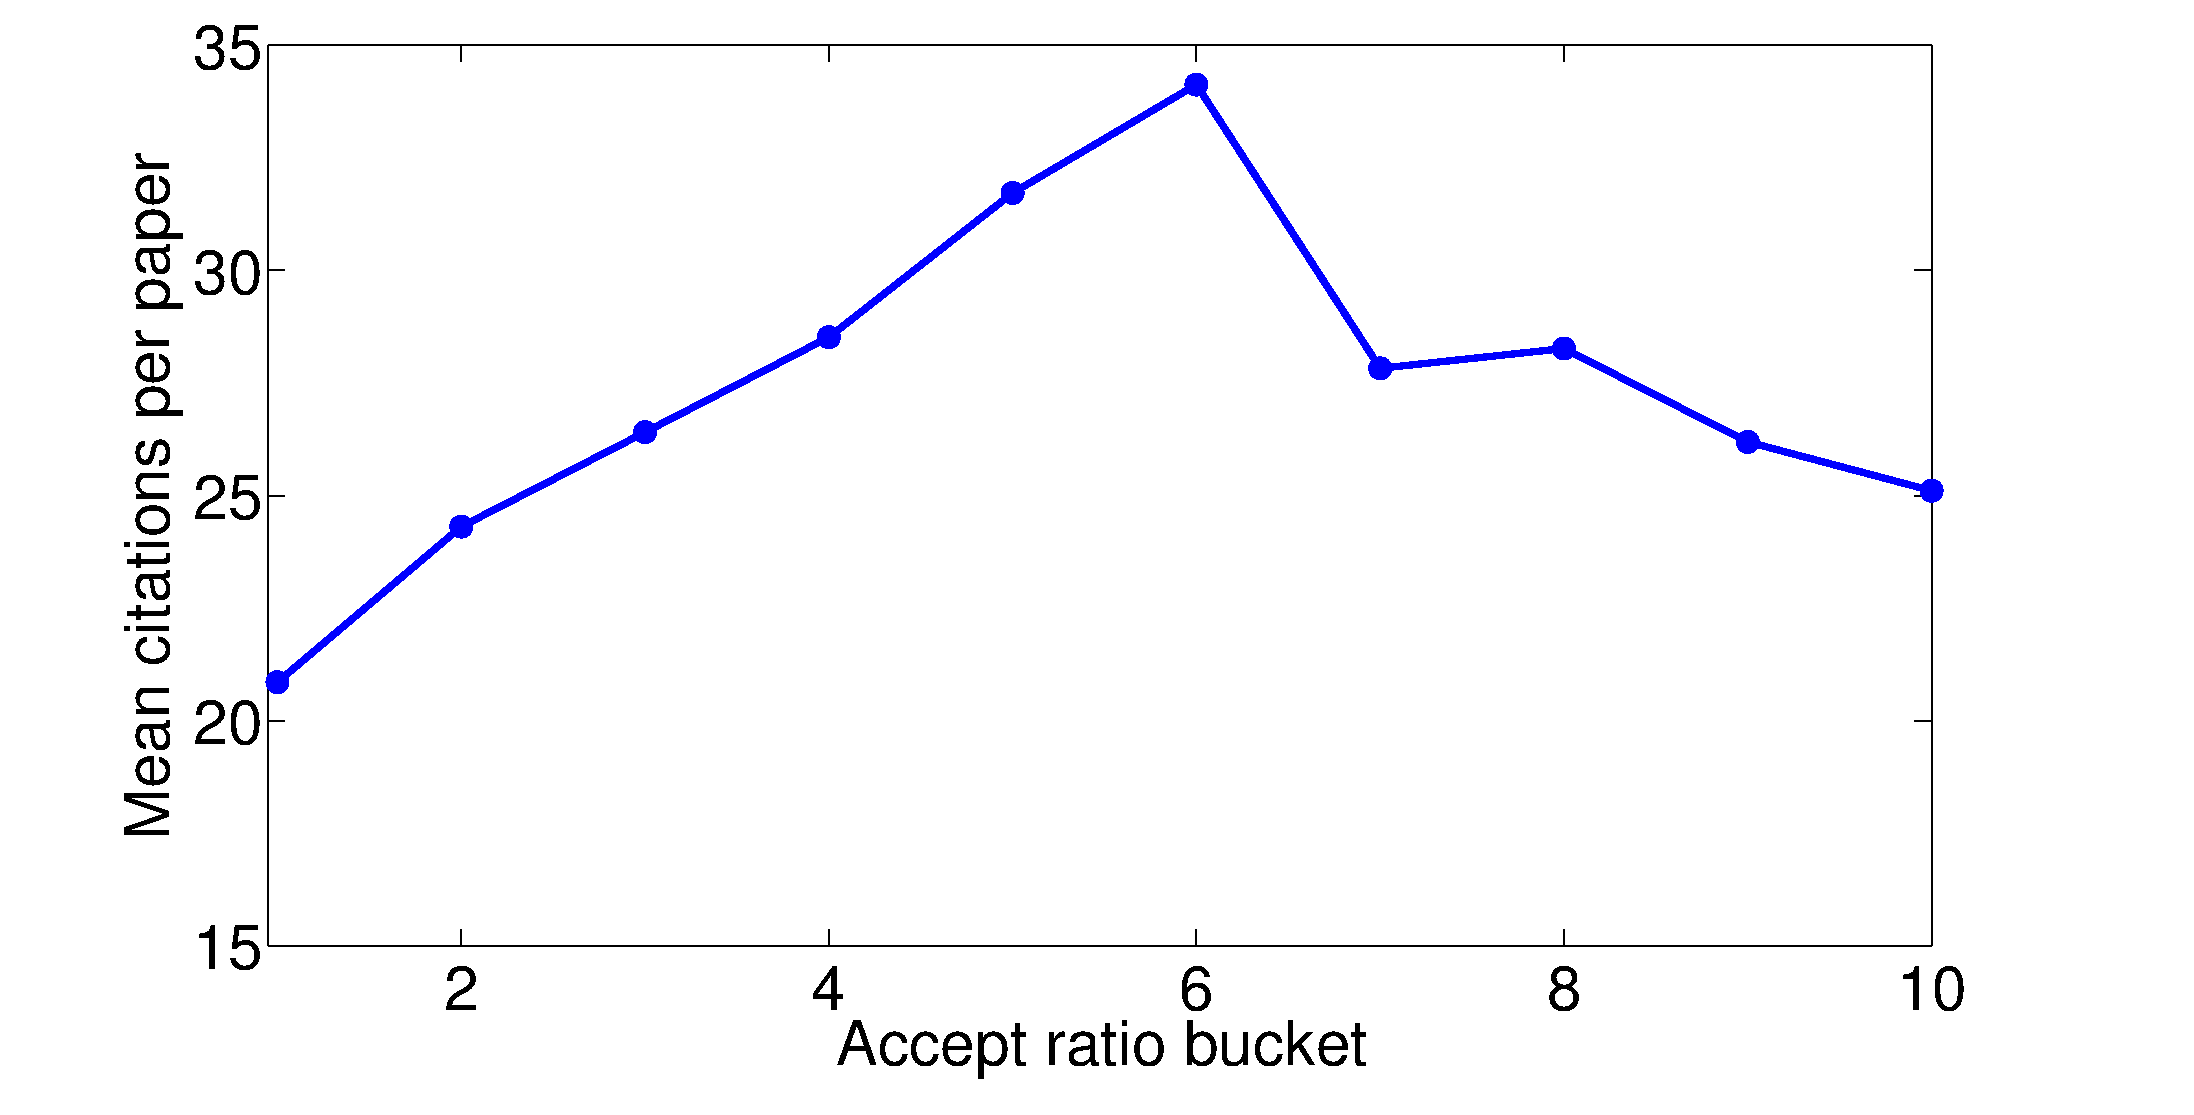
\includegraphics[scale=0.15]{figures/reviewer_citation_ratio-eps-converted-to.pdf} & 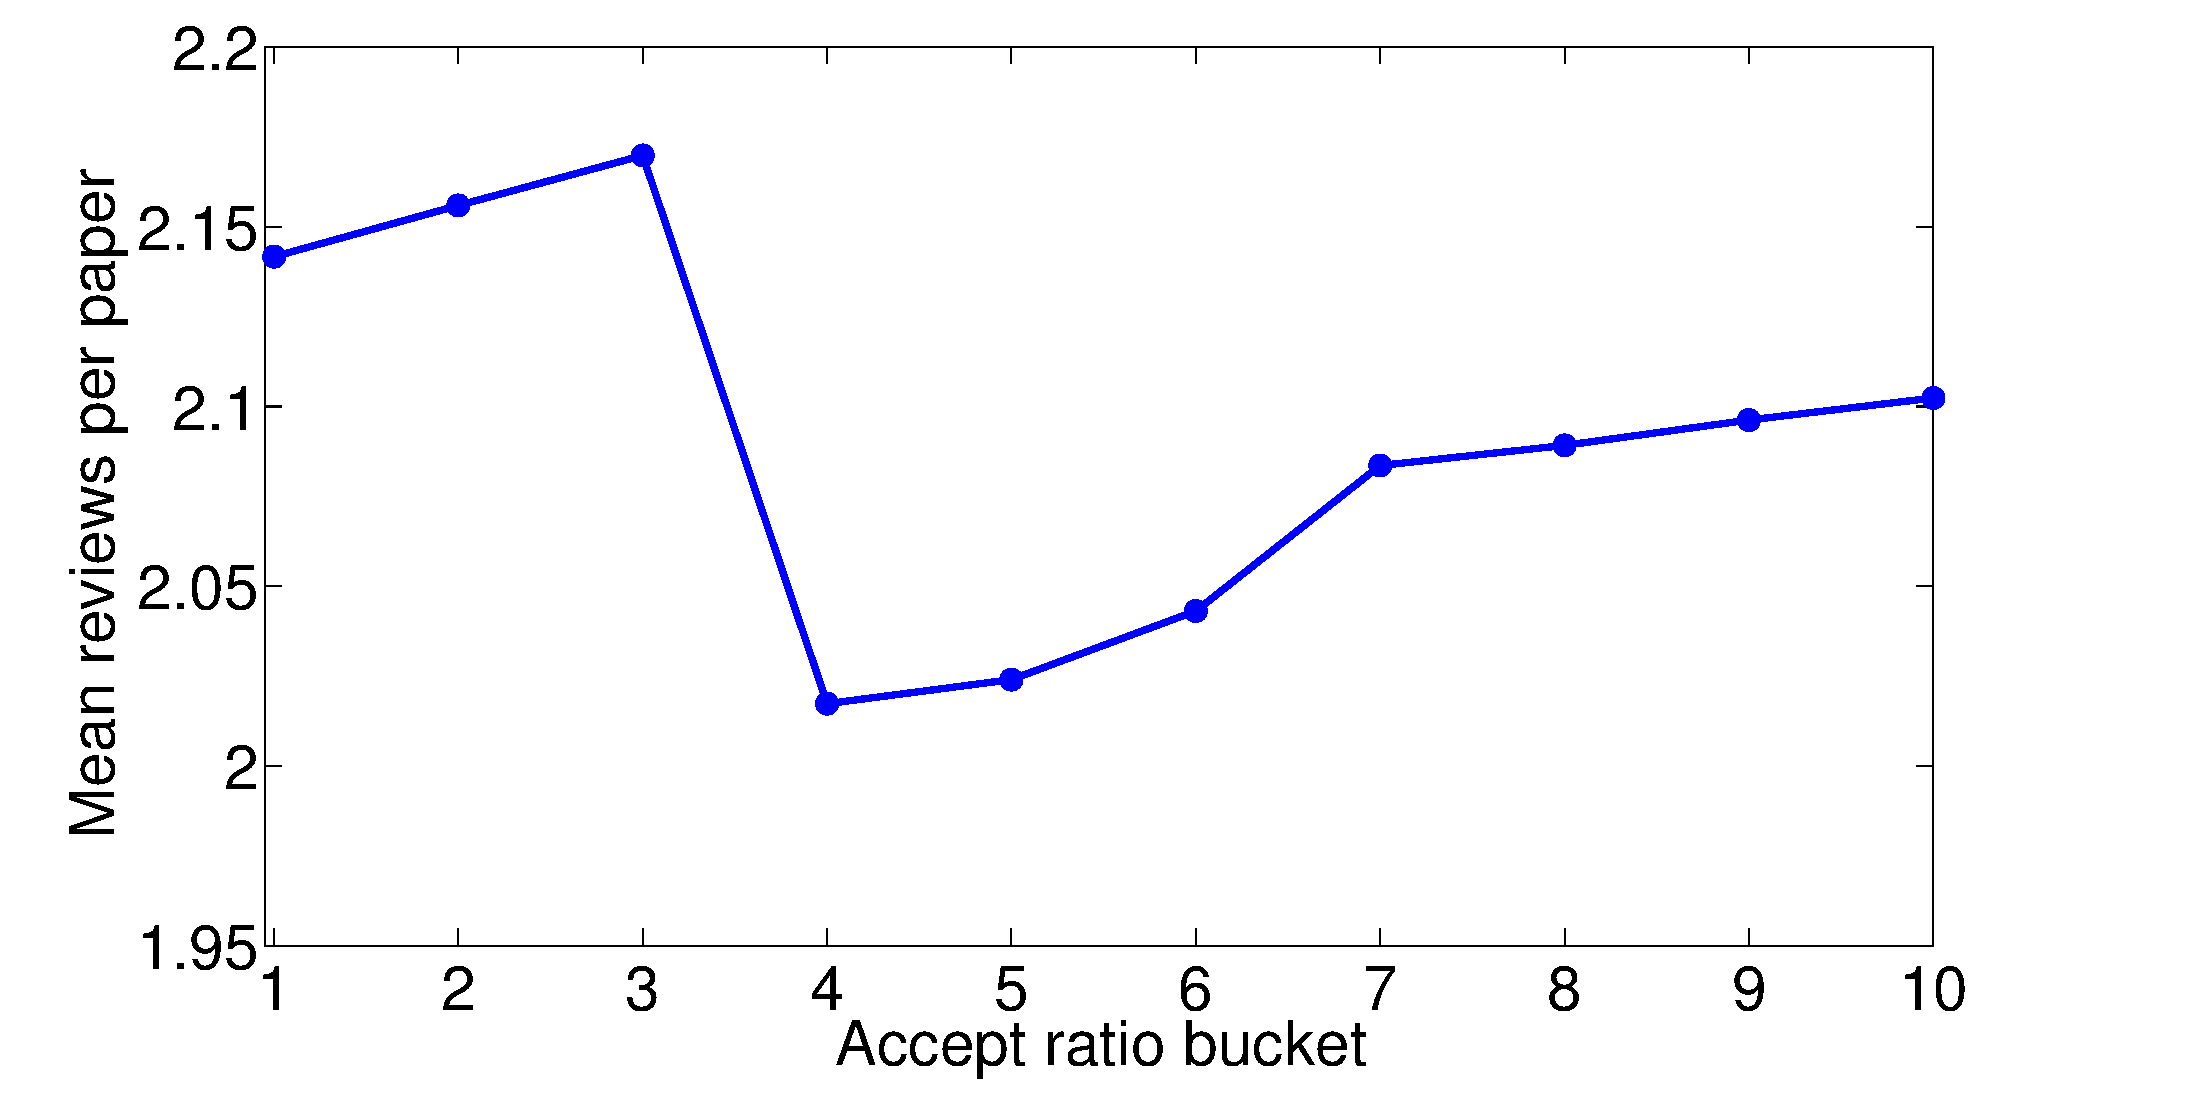
\includegraphics[scale=0.15]{figures/reviewer_review_ratio-eps-converted-to.pdf} & 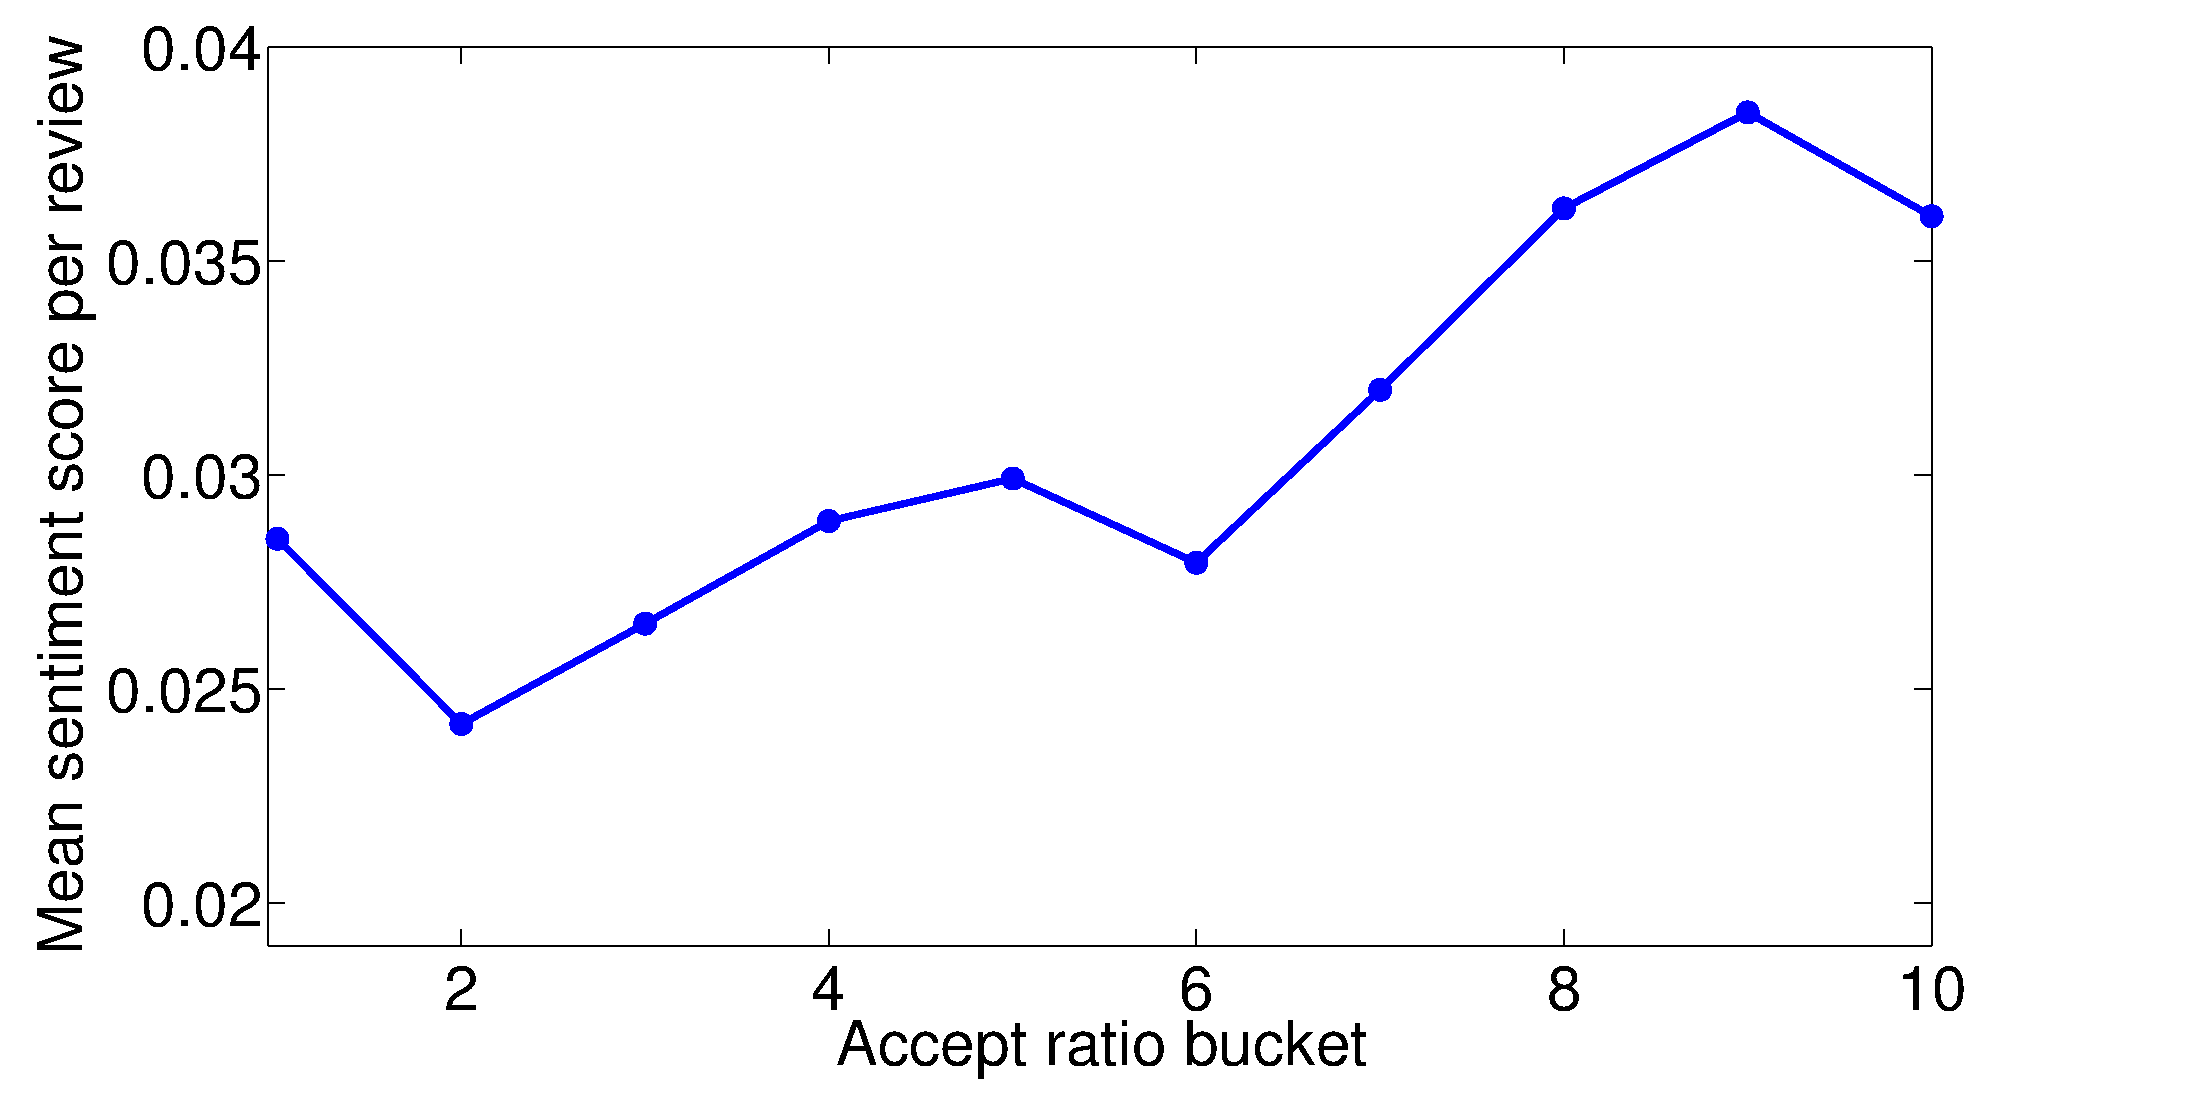
\includegraphics[scale=0.15]{figures/reviewer_sentiment_ratio-eps-converted-to.pdf}
\end{tabular}
\caption{{\bf (Left)} Mean number of citations per paper versus accept ratio. {\bf (Middle)} Mean number of reviews per paper versus accept ratio. {\bf (Right)} Mean sentiment score per paper versus accept ratio. Note that in each case we use accept ratio buckets where the buckets correspond to accept ratio ($\geq 0.1$ and $< 0.2$), ($\geq 0.2$ and $<0.3$) and so on.}
\label{fig16}
%\vspace{-3mm}
\end{figure*}


We start by investigating how well the reviewers were able to anticipate the quality of the paper. To this aim we segregate papers based on their assigned reviewer's accept ratio and calculate the mean number of citations received. In fig.~\ref{fig16}{\bf (Left)} we plot the number of citations per paper given the accept ratio of the assigned reviewer. We observe that most cited papers were reviewed by reviewers with accept ratio between 0.6 and 0.7. Surprisingly, the papers reviewed by reviewers with very low and very high accept ratio tend to garner less citations. This indicates that some papers could have been accepted just because the assigned reviewer is oriented to accept most of the papers. In fact, manual inspection indicates that many of the rejected papers that garnered large number of citations later on were mostly reviewed by reviewers with low accept ratio. We further investigate the number of reviews a reviewer with a given accept ratio suggests before he accepts or rejects a paper. For this we again segregate the papers based on the assigned reviewers accept ratio and calculate the number of rounds of reviews, these papers received on average. We present the results in fig.~\ref{fig16}{\bf (Middle)}. Since in most of the cases the same reviewer is assigned in each round of review, we observe that reviewers with a low accept ratio tend to recommend more rounds of reviews while those with higher accept ratio tend to suggest lesser number of review rounds. This indicates that the reviewers with low accept ratio often fail to improve the quality of the paper as is evident from the mean number of citations these papers receive albeit dragging the paper through multiple rounds of reviews.


To complete the analysis we also investigate the average sentiment score of the papers based on the accept ratio of the assigned reviewers. In fig.~\ref{fig16}{\bf (Right)} we plot the average sentiment score of the papers with similar accept ratio of the assigned reviewer. We observe an increasing trend indicating that the reviewers with very high accept ratio always tend to give more positive reviews as compared to others with lower accept ratio. \iffalse Note that we also repeat the analysis for the small set of editors separately; in all cases the results show exactly similar trends as in case of reviewers.\fi 


\begin{figure}
\centering
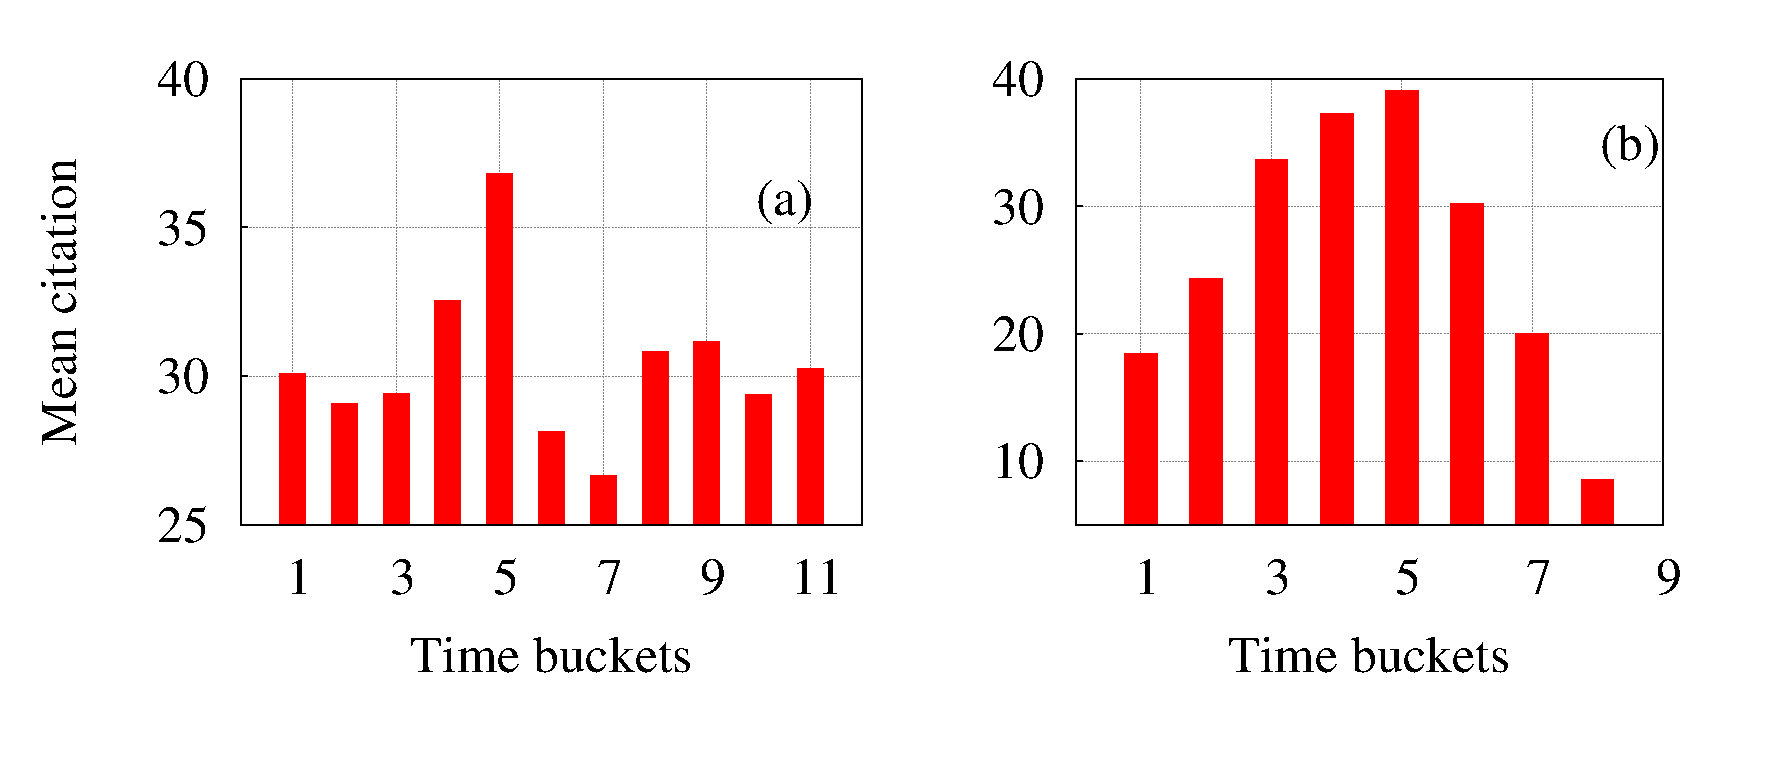
\includegraphics[scale = 0.28]{figures/rev_all.eps}
\caption{\label{fig:rev} Mean citation of the papers versus (a) time since the last assignment for the assigned reviewer and (b) time taken by the reviewer to send the report. Note that for both the cases the times are divided into equi-sized buckets. For (a) bucket sizes are 100 each while for (b) it is 25.}
\end{figure}

\subsubsection{Time since last assignment (TA)}

In lines of~\cite{sikdar2016anomalies} we consider the time (in number of days) since the last assignment for the assigned reviewer as an indicator of reviewer's performance and hence an indicator of the long-term citation of the paper. To verify our hypothesis we segregate the papers based on the assigned reviewer's time till last assignment and calculate the mean citation. The times are bucketed with bucket size typically $< 100$, ($\geq 100, < 200$) and so on. We observe in fig.~\ref{fig:rev}(a) that there does exist an optimal time for which the citation of the accepted paper is maximum. Further if the time since last assignment is too low or too high the long-term citation is low.   

\subsubsection{Delay in submitting the report (DR)}

We further check whether the time taken by the assigned reviewer in submitting the report is also as an indicator for his performance and hence that of the long-term citation of the paper. To this aim we calculate for each paper the time between assigned reviewer acknowledging to review the paper and the reviewer sending back the report. The papers are segregated based on this time and then the mean citation is calculated. 
The times were binned with typical bucket sizes being $>25$, $(\geq 25, < 50)$ and so on. We observe from fig.~\ref{fig:rev}(b) that the citation is maximum when the reviewer sent back the report between 50 and 75 days. The citations are comparatively less if the time is too high as well as too low. 

\medskip